\documentclass[10pt]{article}
%\usepackage{amsmath}
\usepackage{amssymb}
\usepackage{ifthen}
\usepackage{graphicx}
%\usepackage{tikz}
%\usepackage{layout}
\usepackage[textwidth=7.5in,textheight=9.5in]{geometry}
\pagestyle{empty}


\ifthenelse{\boolean{xetex}}%
	{\sffamily
	%%\usepackage{fontspec}
	\usepackage{mathspec}
	\setallmainfonts[Mapping=tex-text]{Calibri}
	\setmainfont[Mapping=tex-text]{Calibri}
	\setsansfont[Mapping=tex-text]{Calibri}
	\setmathsfont(Greek){[cmmi10]}}
	{}
	

\begin{document}
From Caclulus II:\\

%\noindent\begin{minipage}[t]{.7\linewidth}
\textbf{Shell Method:} In Part (a), we have the curve $y=1/(1+x^2)$ drawn from $x=0$ to $x=1$ with the area underneath filled in. This region is then rotated around the $y$-axis, forming a solid in space shown in (b). It would be great to have an interactive element in the text where the reader could watch, or make, this region rotate around the axis.

Also in part (a) is a red rectangle. As the region revolves around the axis, this rectangle forms a ``cylindrical shell'' shown in (c). Watching this rectangle rotate, forming the shell, would also be good. In fact, being able to toggle the region On/Off and the shell On/Off would be great, so a student could watch either one rotate, or both at the same time.
%\end{minipage}
%\begin{minipage}[t]{.3\linewidth}
%\vskip 0pt
%\begin{tabular}{c}
%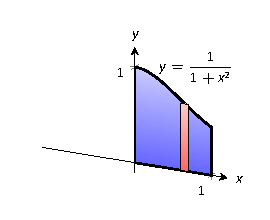
\includegraphics{figures/figshell_intro_b}\\
%(a)\\
%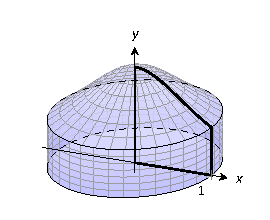
\includegraphics{figures/figshell_intro_a}\\
%(b)\\
%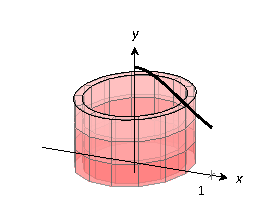
\includegraphics{figures/figshell_intro_d}\\
%(c)
%\end{tabular}

%\end{minipage}

\begin{tabular}{ccc}
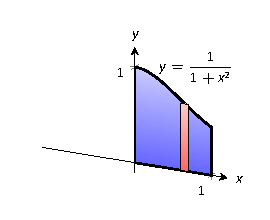
\includegraphics{figures/figshell_intro_b}&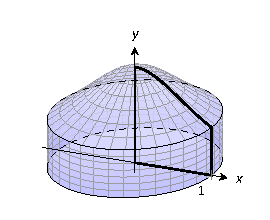
\includegraphics{figures/figshell_intro_a}&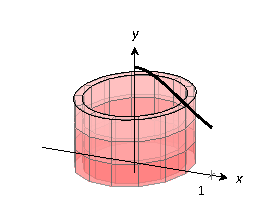
\includegraphics{figures/figshell_intro_d}\\
(a) &(b) & (c)
\end{tabular}

\vskip .5in

From Calculus III:\\

\textbf{Cylinders:} In part (a), the curve $z=y^2$ is drawn (it lies in the $y$-$z$ plane) from $y=-1$ to $y=1$. In part (b), lines are added that go through the curve, each which is parallel to the $x$-axis. Perhaps an animation showing these being drawn would be good. If ``all'' such possible lines are drawn, a surface is created, shown in (c). Another animation showing the spaces between the lines being filled in would be great.

All of this should be done in a 3D environment that can be manipulated to view from various angles/perspectives. 

\begin{tabular}{ccc}
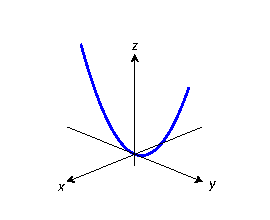
\includegraphics[scale=1.25,trim=5mm 5mm 5mm 5mm,clip=true]{figures/figspace4a} &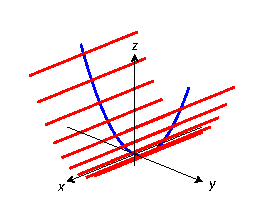
\includegraphics[scale=1.25,trim=5mm 5mm 5mm 5mm,clip=true]{figures/figspace4b} &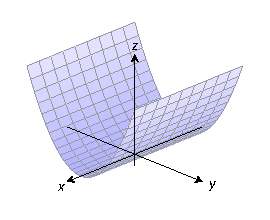
\includegraphics[scale=1.25,trim=3mm 5mm 3mm 2mm,clip=true]{figures/figspace4c}\\[-10pt]
(a) & (b) & (c)
\end{tabular}

Another ``difficult'' example is $x=\sin z$, shown below. Here the red lines are parallel to the $y$-axis. It can be hard to discern in (b) what is going on, although being able to manipulate this in a 3D environment would make it much easier. In (c) again we fill in the spaces to form a solid.

\begin{tabular}{ccc}
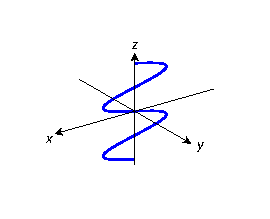
\includegraphics[scale=1.25,trim=5mm 5mm 5mm 5mm,clip=true]{figures/figspace4d} &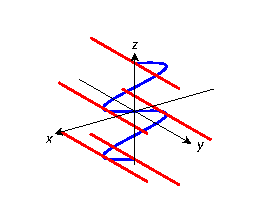
\includegraphics[scale=1.25,trim=5mm 5mm 5mm 5mm,clip=true]{figures/figspace4e} &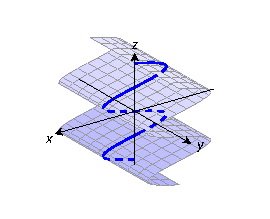
\includegraphics[scale=1.25,trim=5mm 5mm 5mm 5mm,clip=true]{figures/figspace4f}\\[-10pt]
(a) & (b) & (c)
\end{tabular}

\clearpage

Finally, below the surface $z = \sin x\cos y $ is drawn for about $0\leq x\leq 4$, $0\leq y\leq 4$ from two different perspectives.  In each, the level curve $z=\sqrt{3}/4$ is drawn in blue (it is roughly a circle that goes around the ``hill'') and three vectors are plotted. All start at the point $(\pi/3,\pi/3,\sqrt{3}/4 \approx (1.05,1.05, 0.433)$. The dashed vector points to the point $(1.36,0.098,0.433)$. One of the other vectors points to $(1.36,0.098, 1.22)$, the other points to $(2,1.37, .433)$. (The first should look tangent to the surface; the second should be tangent to the surface and also the curve shown in blue.)

Again, it would be great if the environment were interactive and one could view the surface from any perspective. Also, the aspect ratio here is important; The vector pointing to $(1.36,0.098,0.433)$ should look perpendicular to the vector pointing to $(1.36,0.098, 1.22)$.

\begin{tabular}{ccc}
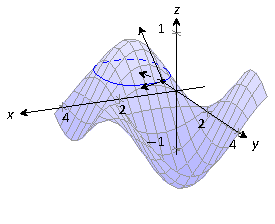
\includegraphics[scale=1.5,trim = 0mm 5mm 0mm 0mm,clip]{figures/figdirect2}& & 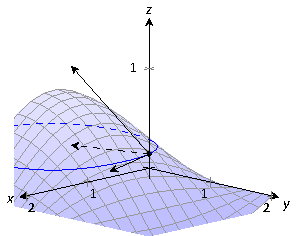
\includegraphics[scale=1.5]{figures/figdirect2b}\\
(a)&\quad  & (b)\\
\end{tabular}


\textbf{Video Content:}\\

It is harder to match content in the book with existing videos as everyone does different examples. The two below fit the subject matter of Chapter 4, Sections 2 and 3, respectively. You could place these videos in the text in a place you deem appropriate.

Related Rates: http://www.youtube.com/watch?v=Xe6YlrCgkIo

Optimization: http://www.youtube.com/watch?v=dam16G6cZ8k



\end{document}